% ------------------------------------------------------------------------------
% TYPO3 Version 10 LTS - What's New (French Version)
%
% @license	Creative Commons BY-NC-SA 3.0
% @link		https://typo3.org/help/documentation/whats-new/
% @language	French
% ------------------------------------------------------------------------------

\section{Interface Utilisateur Backend}
\begin{frame}[fragile]
	\frametitle{Interface Utilisateur Backend}

	\begin{center}\huge{\color{typo3darkgrey}\textbf{Interface Utilisateur Backend}}\end{center}
	\begin{center}\large{\textit{L'interface d'administration de TYPO3 meilleure que jamais}}\end{center}

\end{frame}

% ------------------------------------------------------------------------------
% ...

\begin{frame}[fragile]
	\frametitle{Interface Utilisateur Backend}
	\framesubtitle{Ajustements de l'interface Backend}

	Interface de la colonne des modules backend légèrement altérée.

	\begin{figure}
		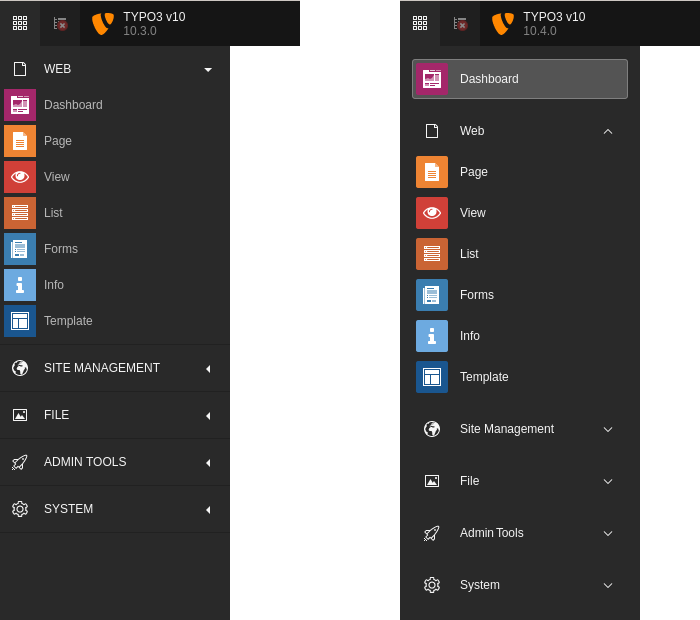
\includegraphics[width=0.5\linewidth]{BackendUserInterface/typo3-backend-ui.png}
	\end{figure}

\end{frame}

% ------------------------------------------------------------------------------
% Feature | 56213 | Allow sorting file list by file meta data title

\begin{frame}[fragile]
	\frametitle{Interface Utilisateur Backend}
	\framesubtitle{Tri de la liste de fichiers}

	Les fichiers peuvent être triés par leur métadonnée «~titre~» depuis le contenu de type
	«~Liste de fichiers~».

	\begin{figure}
		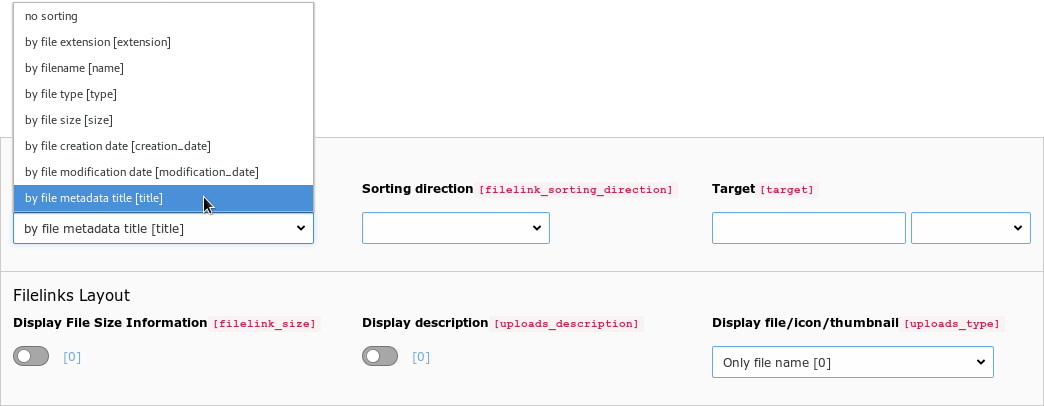
\includegraphics[width=0.90\linewidth]{BackendUserInterface/56213-FilelistSorting.png}
	\end{figure}

\end{frame}

% ------------------------------------------------------------------------------
% Feature | 85569 | Show scheduler information in the system information toolbar

\begin{frame}[fragile]
	\frametitle{Interface Utilisateur Backend}
	\framesubtitle{Barre d'informations système}

	La barre d'information système permet de consulter les informations liées au planificateur TYPO3.

	\begin{figure}
		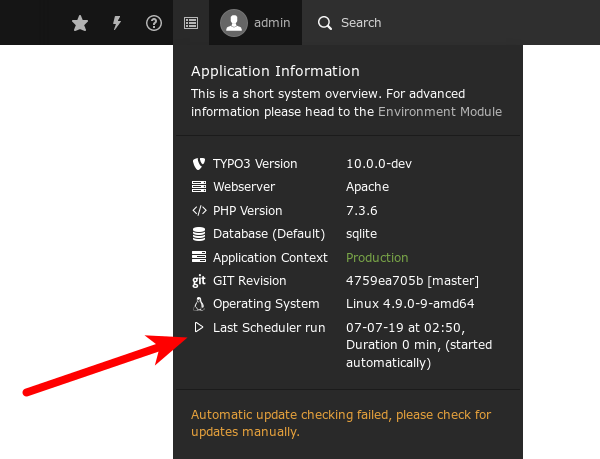
\includegraphics[width=0.50\linewidth]{BackendUserInterface/85569-SchedulerInfoInStatusBar.png}
	\end{figure}

\end{frame}

% ------------------------------------------------------------------------------
% Feature | 86629 | Implement LinkHandler for telephone numbers

\begin{frame}[fragile]
	\frametitle{Interface Utilisateur Backend}
	\framesubtitle{Gestionnaire de lien}

	Un nouveau gestionnaire de lien est ajouté et permet aux utilisateurs Backend de lier des numéros de
	téléphone grâce au protocole \texttt{tel:}.

	\begin{figure}
		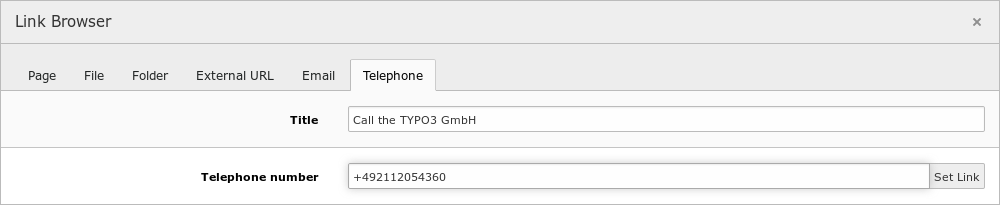
\includegraphics[width=0.90\linewidth]{BackendUserInterface/86629-TelephoneNumberLinkHandler.png}
	\end{figure}

	\begin{figure}
		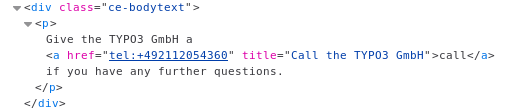
\includegraphics[width=0.60\linewidth]{BackendUserInterface/86629-TelephoneNumberLinkHandler2.png}
	\end{figure}

\end{frame}

% ------------------------------------------------------------------------------
% Feature | 87433 | Add changefreq and priority

\begin{frame}[fragile]
	\frametitle{Interface Utilisateur Backend}
	\framesubtitle{\texttt{EXT:seo}: Vue backend}

	L'extension système \texttt{EXT:seo} supporte le changement des fréquences et priorités de mise à jour pour la Sitemap.
	Les propriétés de page (onglet «~SEO~») fournissent deux nouveaux champs.

	\begin{figure}
		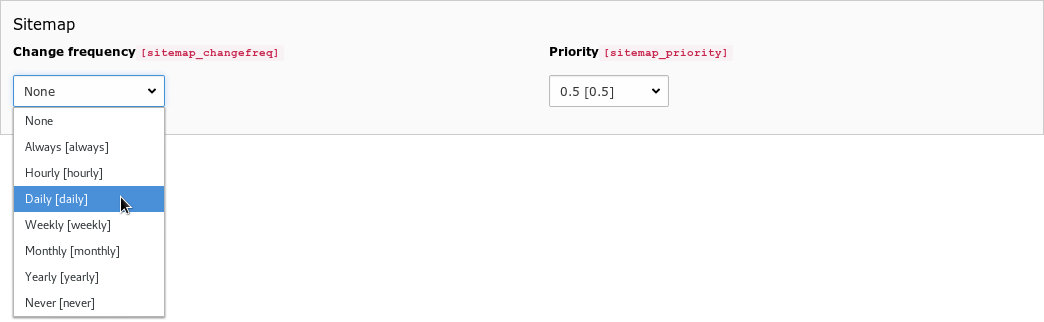
\includegraphics[width=0.90\linewidth]{BackendUserInterface/87433-SeoAddChangefreqAndPriority.png}
	\end{figure}

\end{frame}

% ------------------------------------------------------------------------------
% Feature | 87433 | Add changefreq and priority

\begin{frame}[fragile]
	\frametitle{Interface Utilisateur Backend}
	\framesubtitle{\texttt{EXT:seo}: Options de configuration pour les intégrateurs}

	% decrease font size for code listing
	\lstset{basicstyle=\tiny\ttfamily}

	Ces paramètres peuvent aussi être définis en TypoScript, associés aux champs en base de données.

	\begin{lstlisting}
plugin.tx_seo {
  config {
    xmlSitemap {
      sitemaps {
        <unique key> {
          provider = TYPO3\CMS\Seo\XmlSitemap\RecordsXmlSitemapDataProvider
          config {
            ...
            changeFreqField = news_changefreq
            priorityField = news_priority
            ...
          }
        }
      }
    }
  }
}
	\end{lstlisting}

\end{frame}

% ------------------------------------------------------------------------------
% Feature | 83128 | Content Element Filter

\begin{frame}[fragile]
	\frametitle{Interface Utilisateur Backend}
	\framesubtitle{Recherche dans Nouveau contenu}

	Lors de la création d'un contenu à l'aide de l'assistant «~Nouvel élément de contenu~»,
	l'utilisateur backend peut chercher le type de contenu~:

	\begin{figure}
		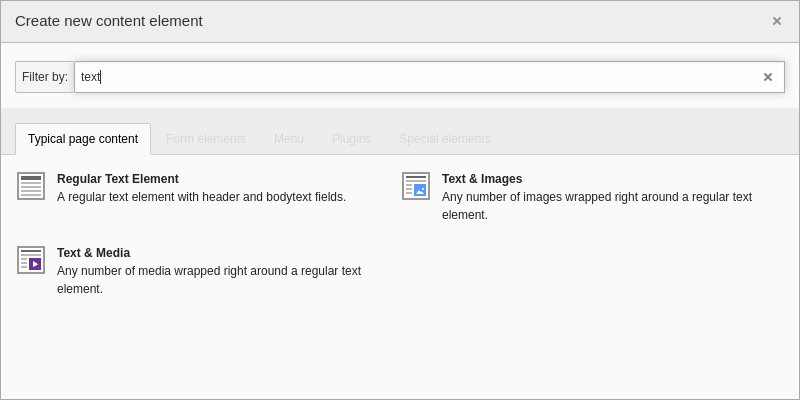
\includegraphics[width=0.6\linewidth]{BackendUserInterface/83128-ContentElementFilter.png}
	\end{figure}

\end{frame}

% ------------------------------------------------------------------------------
% Feature | 85918 | Hide in menu / Show in menu entry for pages in context menu

\begin{frame}[fragile]
	\frametitle{Interface Utilisateur Backend}
	\framesubtitle{Afficher/masquer dans le menu}

	Une nouvelle entrée est ajoutée au menu contextuel pour afficher/masquer les pages.

	\begin{figure}
		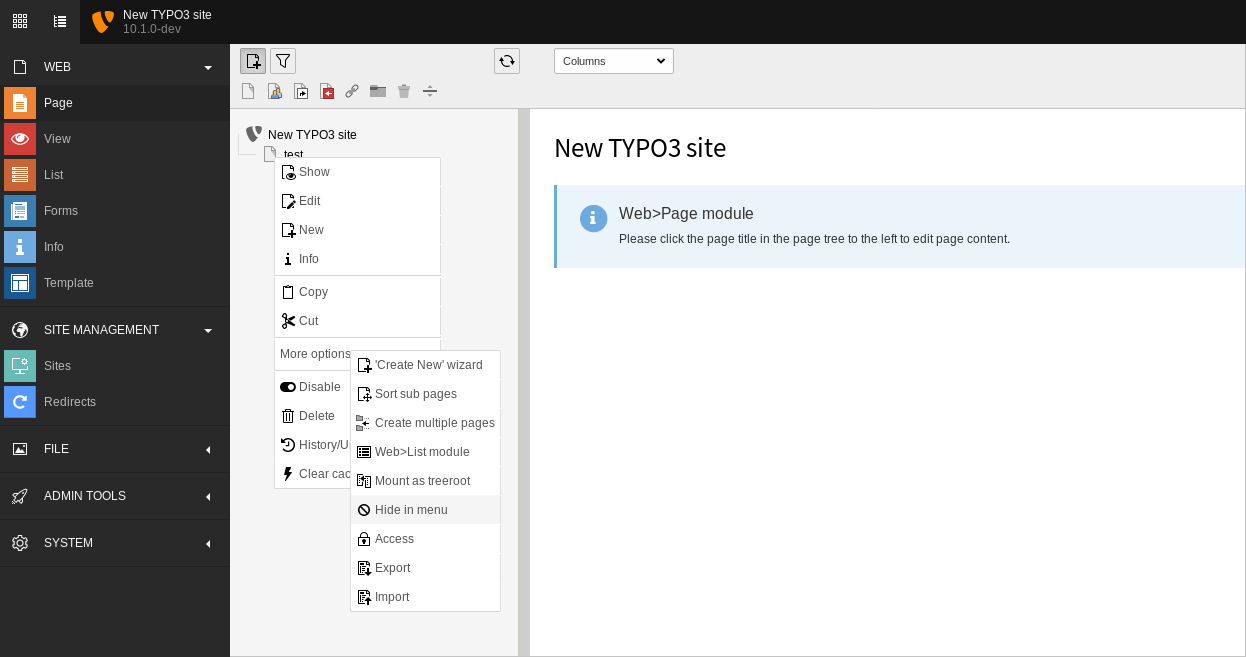
\includegraphics[width=0.80\linewidth]{BackendUserInterface/85918-HideShowInMenu-InContextMenu.png}
	\end{figure}

\end{frame}

% ------------------------------------------------------------------------------
% Feature | 89458 | Show link to online docs in extension manager

\begin{frame}[fragile]
	\frametitle{Interface Utilisateur Backend}
	\framesubtitle{Gestionnaire d'extensions}

	Le gestionnaire d'extension affiche les liens vers la documentation des extensions.

	\begin{figure}
		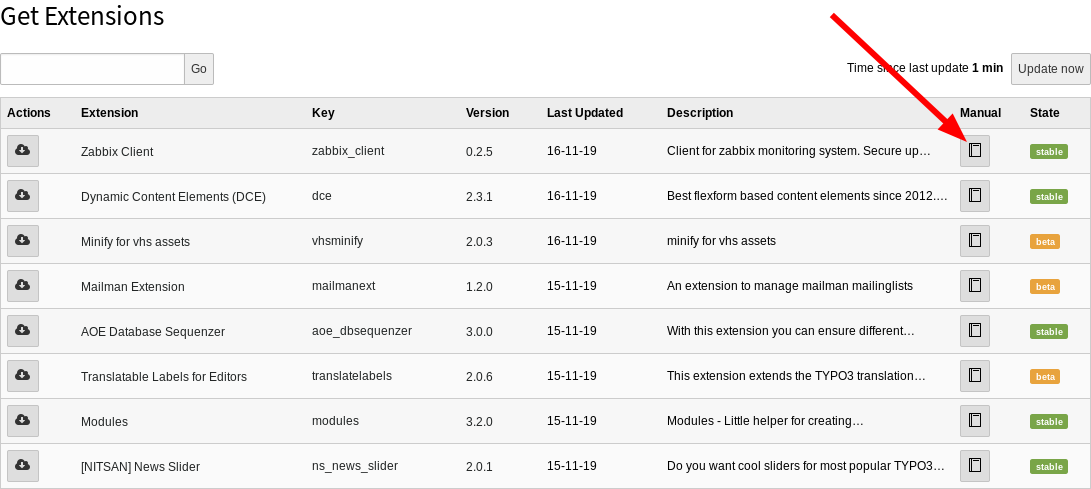
\includegraphics[width=0.90\linewidth]{BackendUserInterface/89458-ShowLinkToOnlineDocsInExtensionManager.png}
	\end{figure}

\end{frame}

% ------------------------------------------------------------------------------
% Feature | 89894 | Separate system extensions from 3rd-party extensions visually

\begin{frame}[fragile]
	\frametitle{Interface Utilisateur Backend}
	\framesubtitle{Gestionnaire d'extensions}

	Les extensions peuvent être filtrées par système et locale dans le gestionnaire d'extensions.

	\begin{figure}
		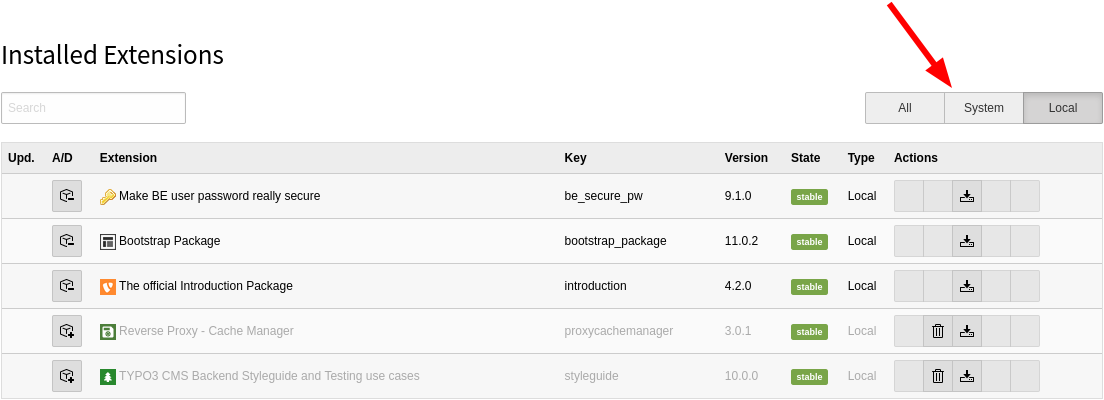
\includegraphics[width=0.9\linewidth]{BackendUserInterface/89894-SeparateSystemExtensionsFrom3rdPartyExtensionsVisually.png}
	\end{figure}

\end{frame}

% ------------------------------------------------------------------------------
% Feature | 86818 | Reintroduce keyboard accessible version of the pagetree

\begin{frame}[fragile]
	\frametitle{Interface Utilisateur Backend}
	\framesubtitle{Accessibilité de l'arborescence des pages}

	Les utilisateurs Backend peuvent naviguer au clavier dans l'arborescence des pages.
	En utilisant les flèches, «~début~», «~fin~», «~entrer~», «~espace~», etc.
	\newline
	Ceci en accord avec les bonnes pratiques décrites dans
	\href{https://www.w3.org/TR/wai-aria-practices-1.1/#keyboard-interaction-22}{WAI-ARIA Authoring Practices 1.1 (en)}
	par le W3C\@.

	\begin{figure}
		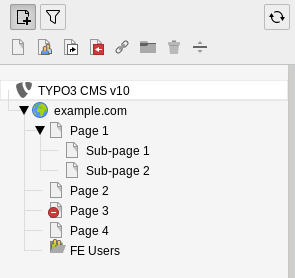
\includegraphics[width=0.30\linewidth]{BackendUserInterface/86818-PagetreeAccessibility.png}
	\end{figure}

\end{frame}

% ------------------------------------------------------------------------------
% Feature | 90298 | Improve user info in BE User module

\begin{frame}[fragile]
	\frametitle{Interface Utilisateur Backend}
	\framesubtitle{Module Utilisateurs backend}

	\begin{itemize}
		\item Une vue détail pour les enregistrements d'utilisateur backend affiche les droits pertinents est ajoutée
		\item Des champs supplémentaires sont ajoutés à la fonction de comparaison des utilisateurs.
		\item Cette fonction prend en compte les sous-groupes.
		\item L'interface utilisateur du module sera encore ajustée et optimisée.
		\item Ces changements facilitent la vérification et la comparaison des permissions des
			utilisateurs sans changer d'utilisateur par les intégrateurs/administrateurs.
	\end{itemize}

\end{frame}

% ------------------------------------------------------------------------------
% Feature | 90826 | Compare backend usergroups

\begin{frame}[fragile]
	\frametitle{Interface Utilisateur Backend}
	\framesubtitle{Module utilisateur backend}

	\begin{itemize}
		\item Les intégrateurs peuvent désormais comparer des groupes d'utilisateurs backend entre eux.
	\end{itemize}

	\begin{figure}
		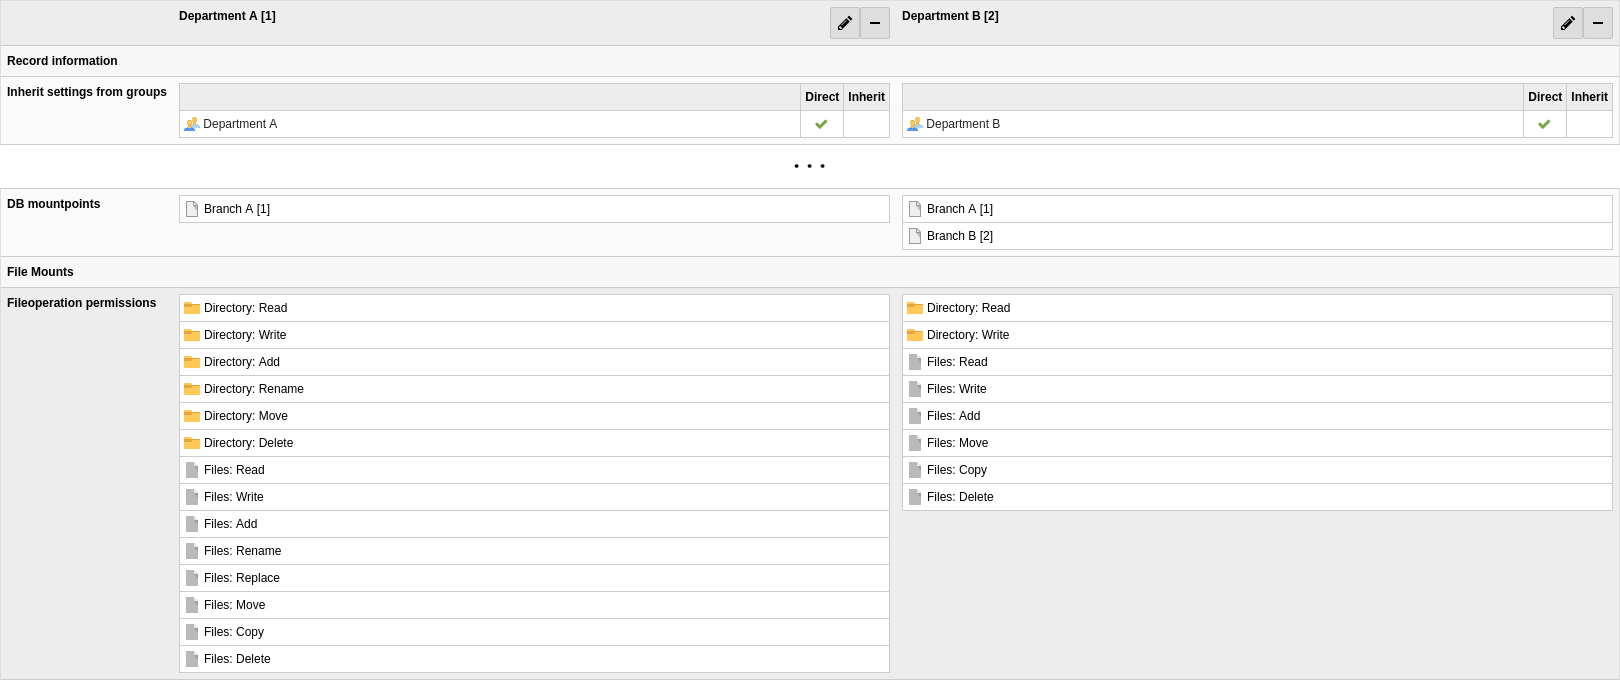
\includegraphics[width=0.9\linewidth]{BackendUserInterface/90826-CompareBackendUsergroups.png}
	\end{figure}

\end{frame}

% ------------------------------------------------------------------------------
% Feature | 90136 | Show application context in the Environment module

\begin{frame}[fragile]
	\frametitle{Interface Utilisateur Backend}
	\framesubtitle{Aperçu de l'environnement}

	Le contexte d'application actuel est affiché dans le module Environnement~:\newline
	\textbf{OUTILS D'ADMINISTRATION} $\rightarrow$ \textbf{Environnement} $\rightarrow$ \textbf{Aperçu de l'environnement}.

	\begin{figure}
		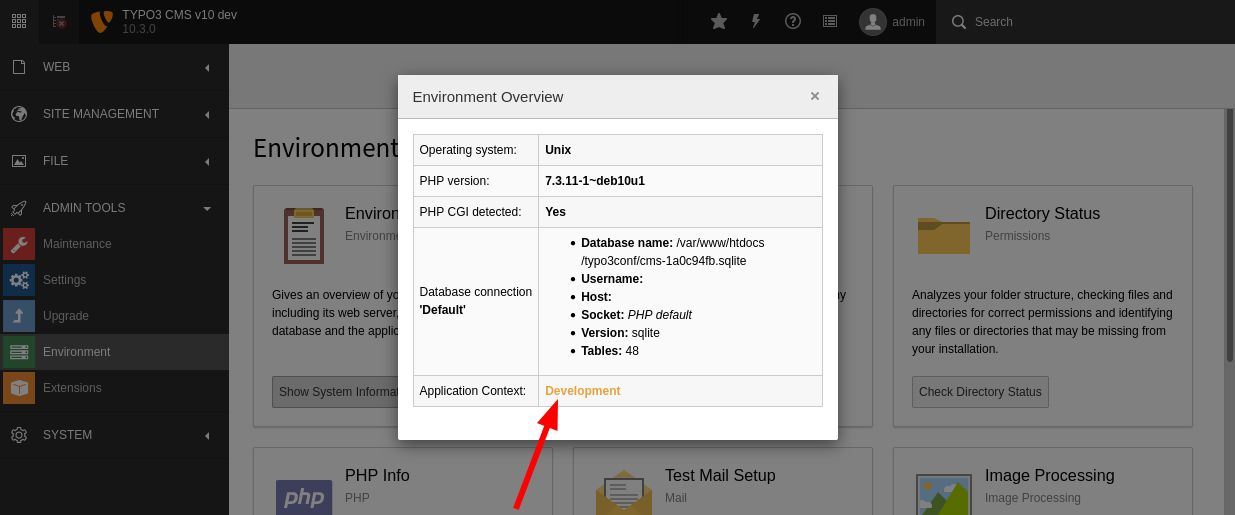
\includegraphics[width=0.9\linewidth]{BackendUserInterface/90136-ShowApplicationContextInTheEnvironmentModule.png}
	\end{figure}

\end{frame}

% ------------------------------------------------------------------------------
% Task | 89844 | Improve visual appearance of feature toggles

\begin{frame}[fragile]
	\frametitle{Interface Utilisateur Backend}
	\framesubtitle{Configuration des fonctionnalités}

	L'apparence visuelle des bascules de fonctionnalité est améliorée~:
	\newline\newline
	\smaller\textbf{TYPO3 v9 LTS}\tabto{6cm}\textbf{TYPO3 v10 LTS}\normalsize

	\begin{figure}
		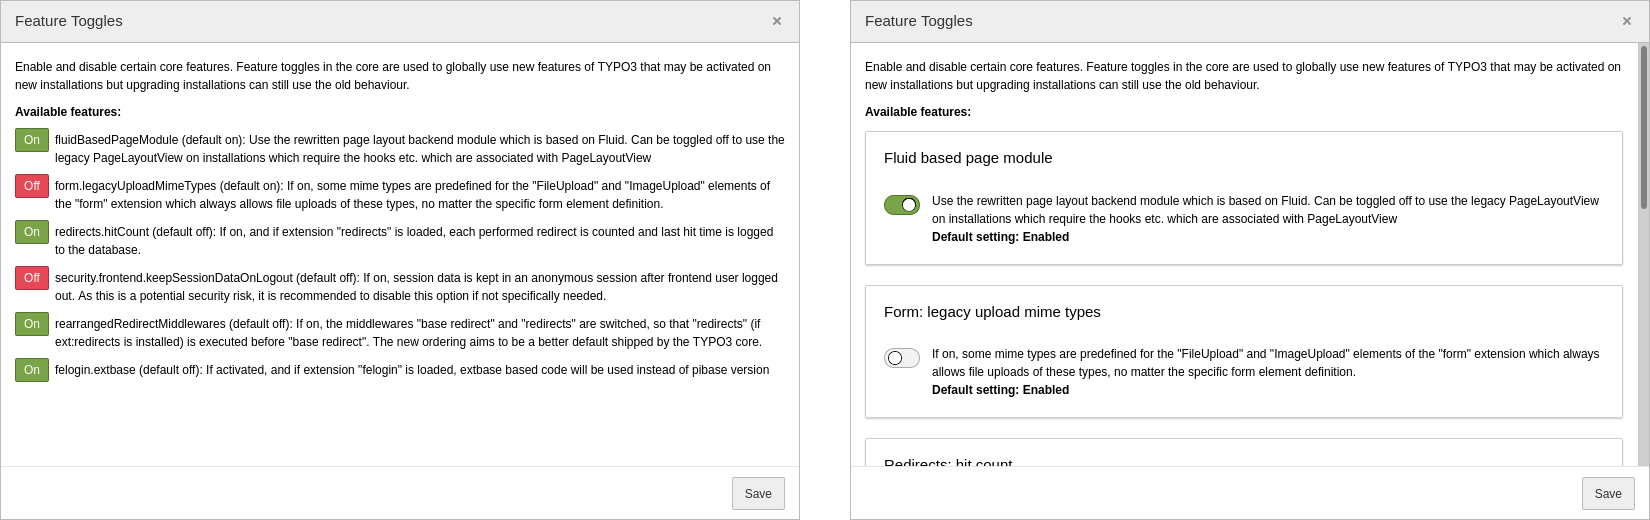
\includegraphics[width=1\linewidth]{InDepthChanges/89844-ImproveVisualAppearanceOfFeatureToggles.png}
	\end{figure}

\end{frame}

% ------------------------------------------------------------------------------
% Feature | 90425 | Add seo fields to info module

\begin{frame}[fragile]
	\frametitle{Interface Utilisateur Backend}
	\framesubtitle{Module Information}

	\begin{itemize}
		\item Les informations SEO et de média sociaux sont affichées dans le module Information~:\newline
			\textbf{WEB} $\rightarrow$ \textbf{Info} $\rightarrow$ \textbf{Aperçu de l'arborescence}.
	\end{itemize}

	\begin{figure}
		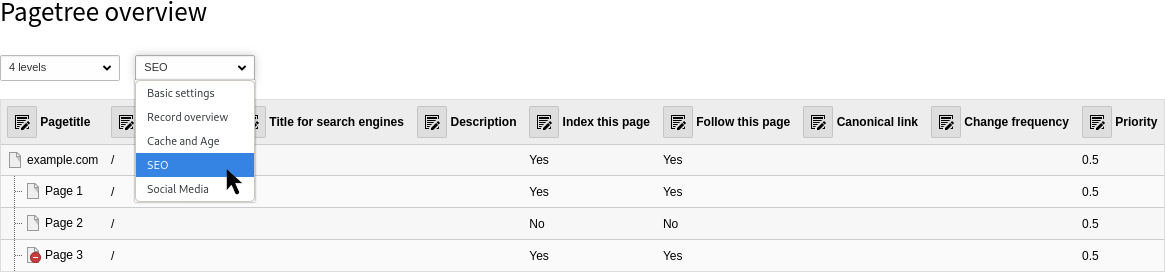
\includegraphics[width=0.85\linewidth]{BackendUserInterface/90425-AddSeoFieldsToInfoModule.png}
	\end{figure}

\end{frame}

% ------------------------------------------------------------------------------
% Feature | 89513 | Provide password recovery for backend users

\begin{frame}[fragile]
	\frametitle{Interface Utilisateur Backend}
	\framesubtitle{Récupération du mot de passe}

	Les utilisateurs backend peuvent réinitialiser leurs informations d'accès en cas d'oubli.

	\begin{figure}
		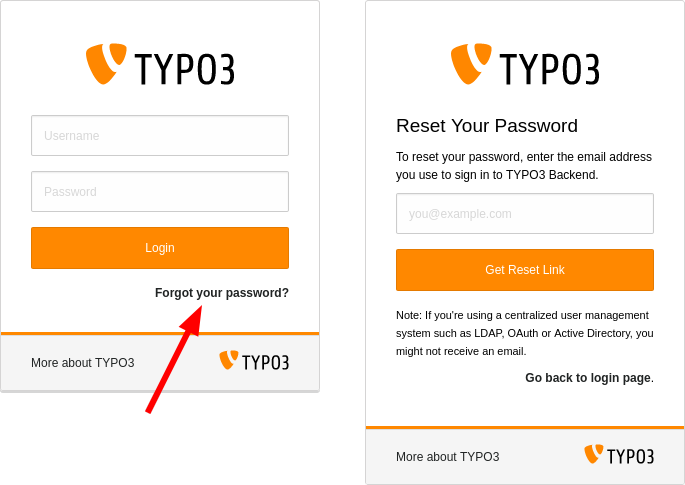
\includegraphics[width=0.55\linewidth]{BackendUserInterface/89513-ProvidePasswordRecoveryForBackendUsers.png}
	\end{figure}

\end{frame}

% ------------------------------------------------------------------------------
% Feature | 89513 | Provide password recovery for backend users

\begin{frame}[fragile]
	\frametitle{Interface Utilisateur Backend}
	\framesubtitle{Réinitialisation du mot de passe d'un utilisateur backend (1)}

	\begin{itemize}

		\item Les liens de réinitialisation de mots de passe ne sont valides que pour 4 heures.\newline
		Cette limite n'est pas configurable.
		\item La fonction est désactivable pour tous les utilisateurs ou seulement les administrateurs pour renforcer la sécurité.
		\item Si des utilisateurs partagent une adresse, un texte alternatif de message est utilisé.
		\item Le champ TCA \texttt{be\_users.email} ne doit pas avoir \texttt{eval=email} de défini.

		\item La fonction ne s'applique que pour les utilisateurs qui~:
			\begin{itemize}
				\item ont une adresse email de définie,
				\item ont un mot de passe de défini, et
				\item ne sont pas désactivé/supprimé.
			\end{itemize}

	\end{itemize}

\end{frame}

% ------------------------------------------------------------------------------
% Feature | 89513 | Provide password recovery for backend users

\begin{frame}[fragile]
	\frametitle{Interface Utilisateur Backend}
	\framesubtitle{Réinitialisation du mot de passe d'un utilisateur backend (2)}

	\begin{itemize}
		\item Il est aussi possible de déclencher la récupération depuis la ligne de commandes.
	\end{itemize}

	\begin{figure}
		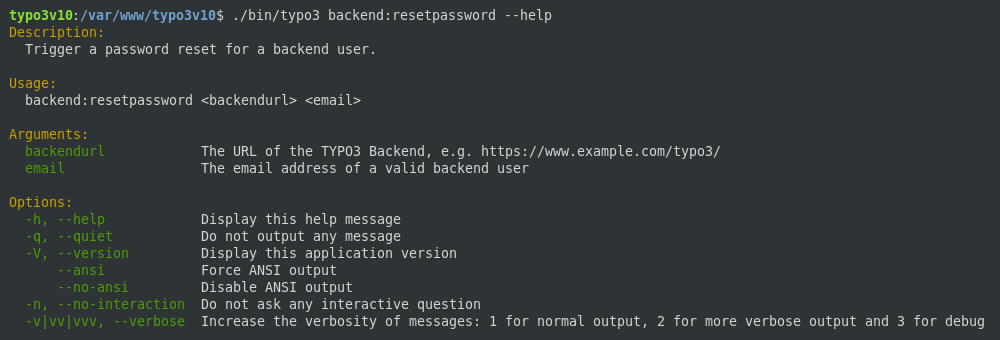
\includegraphics[width=0.9\linewidth]{BackendUserInterface/89513-BackendPasswordResetCommandLine.png}
	\end{figure}

\end{frame}

% ------------------------------------------------------------------------------
% Feature | 89115 | Auto slug update and redirect creation on slug change

\begin{frame}[fragile]
	\frametitle{Interface Utilisateur Backend}
	\framesubtitle{Mise à jour des slugs et des redirections (1)}

	\begin{itemize}
		\item Lorsque les utilisateurs changent le chemin d'URL d'une page (le Slug),
			l'ancienne URL devient inaccessible.
		\item Cela peut générer une erreur «~page non trouvée~» sur la page,
			impactant les URL de ses sous-pages.
	\end{itemize}

	\begin{figure}
		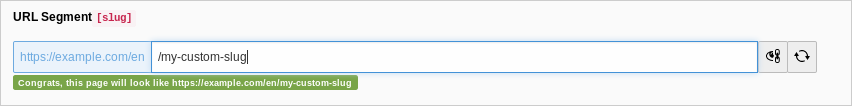
\includegraphics[width=0.80\linewidth]{BackendUserInterface/89115b-AutoSlugUpdateAndRedirectCreationOnSlugChange.png}
	\end{figure}

	\begin{itemize}
		\item Deux actions permettent d'éviter cette erreur~:

			\begin{itemize}
				\item Les slugs des sous-pages sont mises à jour automatiquement
				\item Des redirections de l'ancienne à la nouvelle URL sont créées
			\end{itemize}

	\end{itemize}

\end{frame}

% ------------------------------------------------------------------------------
% Feature | 89115 | Auto slug update and redirect creation on slug change

\begin{frame}[fragile]
	\frametitle{Interface Utilisateur Backend}
	\framesubtitle{Mise à jour des slugs et des redirections (2)}

	\begin{itemize}
		\item Les utilisateurs Backend sont informés de ces actions et peuvent
			facilement revenir en arrière en un clic~:
	\end{itemize}

	\begin{figure}
		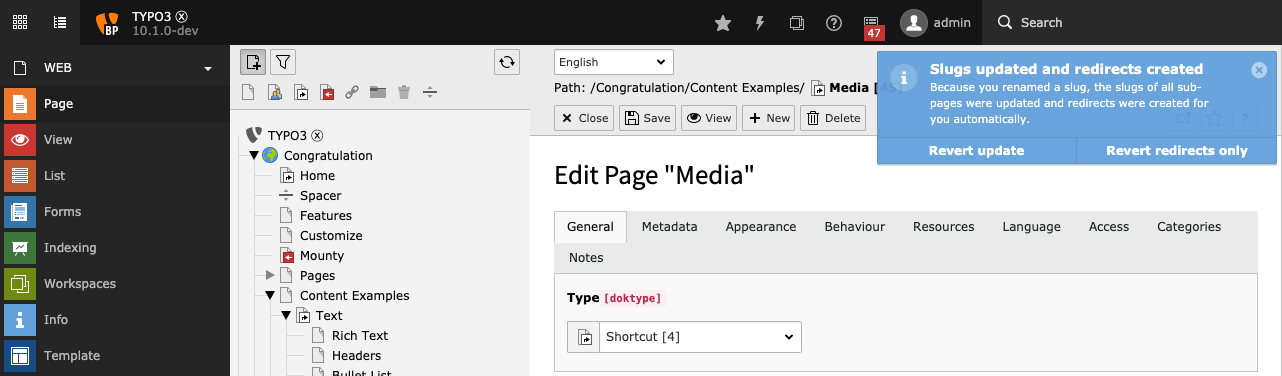
\includegraphics[width=0.80\linewidth]{BackendUserInterface/89115c-AutoSlugUpdateAndRedirectCreationOnSlugChange.png}
	\end{figure}

\end{frame}

% ------------------------------------------------------------------------------
